\chapter{Clasificación a partir de regresión}
Se ha comprobado que usando regresión, se ha conseguido unos buenos modelos para predecir un valor \textbf{preciso} de la intención emprendedora media. El siguiente paso realizado ha sido el de \textbf{categorizar} el caso de regresión, obteniendo así clases del tipo \textit{intención emprendedora alta, baja o media}.\\
Hay que recordar que el resultado obtenido por el modelo de aprendizaje puede ser leído por personal no familiarizado con matemáticas o informática. Este enfoque lo que nos permite es usar una única variable como objetivo con los valores \textit{alto, bajo o alto}, siendo así más legible la salida del algoritmo.
\section{Rendimiento de modelos de clasificación}
Al igual que en los modelos de regresión, en clasificación se hace uso de métricas para ver el comportamiento de los modelos entrenados. A continuación se explica qué métricas se han usado:
\subsection{Accuracy}
Esta métrica mide el porcentaje de casos que el modelo ha clasificado correctamente.
\[
	accuracy(y,\hat{y})=\frac{1}{n_{samples}}\sum_{i=1}^{n_{samples}}1(\hat{y_i}=y_i)
\]

\subsection{Matriz de confusión y métricas}
Cada entrada $i.j$ de la matriz se define como el número de observaciones del grupo $i$ que han sido predichas como del grupo $j$.  Un ejemplo de matriz de confusión para el problema que se esta tratando es:
 \begin{figure}[H]
	\centering
	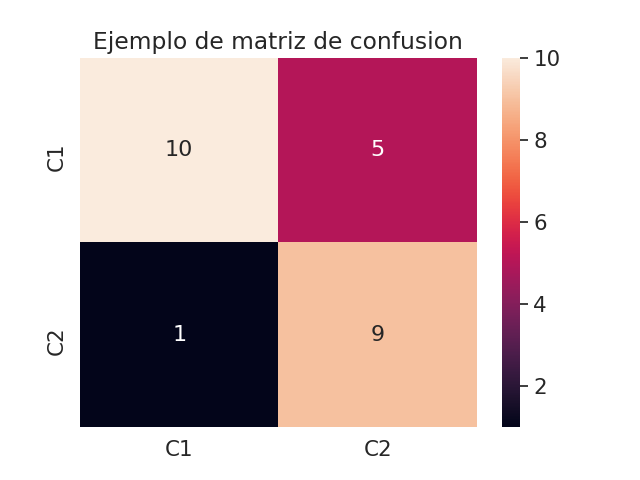
\includegraphics[scale=0.8]{conf_matrix.png}
	\caption{Ejemplo de matriz de confusión}
	\label{fig:conf_matrix}
\end{figure}
Aquí podemos ver cuantas muestras de una clase  el modelo predijo como correctas (de la misma clase) y cuantas muestras de una clase predijo como  erróneas (de distinta clase).\\
\linebreak
A partir de la matriz de confusión, se pueden sacar las siguiente métricas:
 \[Precision = \frac{TP} {TP + FP}\]
 \[Recall = \frac{TP}{TP + FN}\]
 \[FPR = \frac{FP}{FP + TN}\]
 \[ F1\_score = 2 \times \frac{Precision \times Recall}{Precision + Recall} \]
  Intuitivamente, \textbf{Precision} mide la habilidad del modelo de no clasificar como \textbf{positiva} una muestra que es \textbf{negativa}, mientras que \textbf{Recall} mide la habilidad del modelo para clasificar bien todas las muestras positivas.\\
  \linebreak
 Cabe destacar que se han explicado para el caso de clasificación binaria, pero estas métricas se pueden extender para la clasificación multi-clase y multi-etiqueta.
\subsection{Curva ROC y AUC}
Partiendo de lo explicado sobre la matriz de confusión, la curva ROC (Receiver Operating Characteristic Curve) es un gráfico donde se representa el \textbf{FPR} (False Positive Rate) en el eje \textbf{X} y el \textbf{TPR} (True Positive Rate o Recall) en el eje \textbf{Y}. Se escogen estas métricas debido a la siguiente hipótesis:\\
A medida que incrementamos el ratio de verdaderos positivos, se va a incrementar el ratio de falsos positivos debido a que es más probable que el modelo clasifique como positivo una muestra que no es positiva.
 \begin{figure}[H]
	\centering
	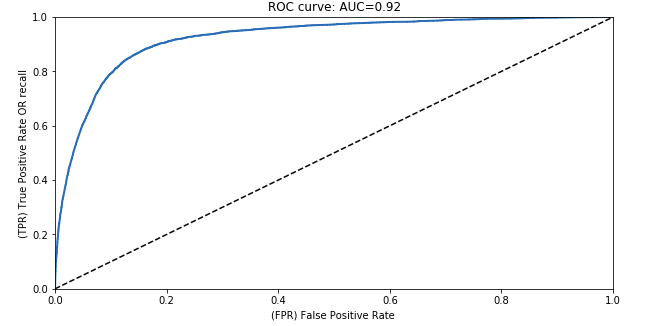
\includegraphics[scale=0.5]{roc}
	\caption{Ejemplo de curva ROC}
	\label{fig:roc}
\end{figure}
Lo ideal, es que la figura se acerque a la esquina superior izquierda lo máximo posible, ya que implicaría que se esta clasificando como correctos todas las muestras positivas y ninguna muestra negativa se está clasificando como positiva.\\
Se puede usar el área bajo la curva  como una métrica para comprobar como de bueno es el modelo. Esta métrica se conoce como \textbf{AUC} (Area Under Curve).\\
\linebreak
Al igual que en regresión (\ref{sec:validation}-\nameref{sec:validation}), se ha usado la técnica de \textit{k-fold validation} para validar el rendimiento de los modelos entrenados.
\section{Modelos de clasificación}
Para clasificación, se van a usar unicamente aquellos modelos que se ha demostrado empíricamente en la sección \ref{sec:algoritmos}-\nameref{sec:algoritmos} que han tenido un buen desempeño. Por tanto se van a usar Árboles de Decisión, Random Forest y SVM.
\subsection{Árboles de Decisión}
En esta sección se va a exponer los resultados obtenidos en clasificación usando  \textbf{Árboles de Decisión}.\\
La siguiente tabla expone los resultados obtenidos:
\begin{table}[H]
	\centering
	\begin{tabular}{|c|c|c|c|c}
		\cline{1-4}
	    FOLD & F1 Score & AUC Score & Accuracy  \\ \cline{1-4}
	    Fold 0 & 0.721 & 0.87 & 0.741 \\ \cline{1-4}
	    Fold 1 & 0.761 & 0.883 & 0.761 \\ \cline{1-4}
	    Fold 2 & 0.695 & 0.84 & 0.725 \\ \cline{1-4}
	    Fold 3 & 0.692 & 0.824 & 0.733 \\ \cline{1-4}
	    Fold 4 & 0.795 & 0.887 & 0.788 \\ \cline{1-4}
	    Fold 5 & 0.733 & 0.861 & 0.75 \\ \cline{1-4}
	    Train & 0.785 & 0.897 & 0.802 \\ \cline{1-4}
	    Test & 0.691 & 0.813 & 0.72 \\ \cline{1-4}
	\end{tabular}
	\caption{Árbol de decisión:  Profundidad 4. número máximo de hojas 16}
	\label{tab:dtree_class_res}
\end{table}
A continuación se muestra la matriz de confusión obtenida por el modelo:
 \begin{figure}[H]
	\centering
	\includegraphics[scale=0.5]{src/confusion_matrix_dtree_classification}
	\caption{Matriz de confusión para Árboles de Decisión}
	\label{fig:confusion_matrix_dtree}
\end{figure}

\subsection{Random Forest}
En esta sección se va a exponer los resultados obtenidos en clasificación usando  \textbf{Random Forest}.\\
La siguiente tabla expone los resultados obtenidos:
\begin{table}[H]
	\centering
	\begin{tabular}{|c|c|c|c|c}
		\cline{1-4}
		FOLD & F1 Score & AUC Score & Accuracy \\ \cline{1-4}
		Fold 0 & 0.751 & 0.887 & 0.773\\ \cline{1-4}
		Fold 1 & 0.803 & 0.914 & 0.809\\ \cline{1-4}
		Fold 2 & 0.734 & 0.881 & 0.749\\ \cline{1-4}
		Fold 3 & 0.69 & 0.838 & 0.725\\ \cline{1-4}
		Fold 4 & 0.739 & 0.905 & 0.772\\ \cline{1-4}
		Fold 5 & 0.743 & 0.885 & 0.766\\ \cline{1-4}
		Train & 0.998 & 1.0 & 0.998\\\cline{1-4}
		Test & 0.737 & 0.891 & 0.766\\\cline{1-4}
	\end{tabular}
	\caption{Árbol de decisión:  Profundidad 4. número máximo de hojas 16}
	\label{tab:rf_class_res}
\end{table}
A continuación se muestra la matriz de confusión obtenida por el modelo:
\begin{figure}[H]
	\centering
	\includegraphics[scale=0.5]{src/confusion_matrix_rf_class}
	\caption{Matriz de confusión para Random Forest}
	\label{fig:confusion_matrix_rf}
\end{figure}


\subsection{Support Vector Machines}
En esta sección se va a exponer los resultados obtenidos en clasificación usando  \textbf{Random Forest}.\\
La siguiente tabla expone los resultados obtenidos:
\begin{table}[H]
	\centering
	\begin{tabular}{|c|c|c|c|c}
		\cline{1-4}
		FOLD & F1 Score & AUC Score & Accuracy \\\cline{1-4}
		Fold 0 & 0.697 & 0.87 & 0.737\\ \cline{1-4}
		Fold 1 & 0.794 & 0.913 & 0.801\\ \cline{1-4}
		Fold 2 & 0.717 & 0.904 & 0.741\\ \cline{1-4}
		Fold 3 & 0.695 & 0.86 & 0.737\\ \cline{1-4}
		Fold 4 & 0.739 & 0.909 & 0.784\\ \cline{1-4}
		Fold 5 & 0.728 & 0.891 & 0.76\\ \cline{1-4}
		Train & 0.925 & 0.989 & 0.932\\\cline{1-4}
		Test & 0.747 & 0.906 & 0.778\\\cline{1-4}
	\end{tabular}
	\caption{Árbol de decisión:  Profundidad 4. número máximo de hojas 16}
	\label{tab:svm_class_res}
\end{table}
A continuación se muestra la matriz de confusión obtenida por el modelo:
\begin{figure}[H]
	\centering
	\includegraphics[scale=0.5]{src/confusion_matrix_rf_class}
	\caption{Matriz de confusión para SVM}
	\label{fig:confusion_matrix_svm}
\end{figure}
\subsection{Conclusiones}
Como se puede apreciar, ninguno de los algoritmos no han tenido problemas clasificando la clase \textbf{IEAlta}, clasificando correctamente más del $80\%$ de las instancias de esta clase.
Los algoritmos han tenido más problemas a la hora de clasificar correctamente la clase \textbf{IEBaja}, clasificando correctamente solo el $50\%$. Volviendo a la figura \ref{tab:ocurrencia_valores} donde se mostraba el conteo de clases, se puede apreciar que la clase formada por los valores más bajos tiene una menor cantidad de muestras, explicando así que los algoritmos fallen más comúnmente en estas clases, clasificando una gran parte como \textbf{IEMedia} (tiene sentido ya que es la clase más 'cercana') .